\documentclass{ConfigurationFiles/PoliMi3i_thesis}


% CONFIGURATIONS
\usepackage{parskip} % For paragraph layout
\usepackage{setspace} % For using single or double spacing
\usepackage{emptypage} % To insert empty pages
\usepackage{multicol} % To write in multiple columns (executive summary)
\setlength\columnsep{15pt} % Column separation in executive summary
\setlength\parindent{0pt} % Indentation
\raggedbottom
\usepackage{multirow}

% PACKAGES FOR TITLES
\usepackage{titlesec}
% \titlespacing{\section}{left spacing}{before spacing}{after spacing}
\titlespacing{\section}{0pt}{3.3ex}{2ex}
\titlespacing{\subsection}{0pt}{3.3ex}{1.65ex}
\titlespacing{\subsubsection}{0pt}{3.3ex}{1ex}
\usepackage{color}

% PACKAGES FOR LANGUAGE AND FONT
\usepackage[english]{babel} % The document is in English  
\usepackage[utf8]{inputenc} % UTF8 encoding
\usepackage[T1]{fontenc} % Font encoding
\usepackage[11pt]{moresize} % Big fonts

% PACKAGES FOR IMAGES
\usepackage{graphicx}
\usepackage{transparent} % Enables transparent images
\usepackage{eso-pic} % For the background picture on the title page
\usepackage{subfig} % Numbered and caption subfigures using \subfloat.
\usepackage{tikz} % A package for high-quality hand-made figures.
\usetikzlibrary{}
\graphicspath{{./Images}} % Directory of the images
\usepackage{amsthm} % Coloured "Theorem"
\usepackage{thmtools}
\usepackage{xcolor}
\usepackage{float}

% STANDARD MATH PACKAGES
\usepackage{amsmath}
\usepackage{amssymb}
\usepackage{amsfonts}
\usepackage{bm}
\usepackage[overload]{empheq} % For braced-style systems of equations.
\usepackage{fix-cm} % To override original LaTeX restrictions on sizes

% PACKAGES FOR TABLES
\usepackage{tabularx}
\usepackage{longtable} % Tables that can span several pages
\usepackage{colortbl}

% PACKAGES FOR ALGORITHMS (PSEUDO-CODE)
\usepackage{algorithm}
\usepackage{algorithmic}


% PACKAGES FOR REFERENCES & BIBLIOGRAPHY
\usepackage[
    colorlinks=true,
    linkcolor=black,
    anchorcolor=black,
    citecolor=black,
    filecolor=black,
    menucolor=black,
    runcolor=black,
    urlcolor=black
]{hyperref} % Adds clickable links at references
\usepackage{cleveref}
\usepackage[square, numbers, sort&compress]{natbib} % Square brackets, citing references with numbers, citations sorted by appearance in the text and compressed
\bibliographystyle{abbrvnat} % You may use a different style adapted to your field

% OTHER PACKAGES
\usepackage{pdfpages} % To include a pdf file
\usepackage{afterpage}
\usepackage{lipsum} % DUMMY PACKAGE
\usepackage{fancyhdr}
\usepackage{wasysym} % For the headers
\usepackage{rotating}
\usepackage{listings}
\usepackage{hyperref}
%%
% Alloy language definition for using with the listings package.
%
% 2017, Daniel Andrade
% BSD 3-Clause License
%%
\lstdefinelanguage{alloy}{
    morekeywords={
        module, open, as,
        private, abstract, sig, extends, in,
        lone, some, one, disj,
        fact, pred, fun, assert,
        run, check,
        for, but, exactly,
        this, not, implies, else, let,
        not, no, set, all, sum,
        iff, or, Int, and,
        none, univ, iden
    },
    sensitive=true,
    morecomment=[l]{//},
    morecomment=[l]{--},
    morecomment=[s]{/*}{*/},
    morestring=[b]{"},
%literate={->}{$\rightarrow$}1
% replacing characters can cause problems when copying from PDF to editor
}[keywords,comments,strings]

\fancyhf{}

% Input of configuration file. Do not change config.tex file unless you really know what you are doing. 
% Define blue color typical of polimi
\definecolor{bluepoli}{cmyk}{0.4,0.1,0,0.4}

% Custom theorem environments
\declaretheoremstyle[
    headfont=\color{bluepoli}\normalfont\bfseries,
    bodyfont=\color{black}\normalfont\itshape,
]{colored}

% Set-up caption colors
\captionsetup[figure]{labelfont={color=bluepoli}} % Set colour of the captions
\captionsetup[table]{labelfont={color=bluepoli}} % Set colour of the captions
\captionsetup[algorithm]{labelfont={color=bluepoli}} % Set colour of the captions

\theoremstyle{colored}
\newtheorem{theorem}{Theorem}[chapter]
\newtheorem{proposition}{Proposition}[chapter]

% Enhances the features of the standard "table" and "tabular" environments.
\newcommand\T{\rule{0pt}{2.6ex}}
\newcommand\B{\rule[-1.2ex]{0pt}{0pt}}

% Pseudo-code algorithm descriptions.
\newcounter{algsubstate}
\renewcommand{\thealgsubstate}{\alph{algsubstate}}
\newenvironment{algsubstates}
{\setcounter{algsubstate}{0}%
\renewcommand{\STATE}{%
    \stepcounter{algsubstate}%
    \Statex {\small\thealgsubstate:}\space}}
{}

% New font size
\newcommand\numfontsize{\@setfontsize\Huge{200}{60}}

% Title format: chapter
\titleformat{\chapter}[hang]{
    \fontsize{50}{20}\selectfont\bfseries\filright}{\textcolor{bluepoli} \thechapter\hsp\hspace{2mm}\textcolor{bluepoli}{|   }\hsp}{0pt}{\huge\bfseries \textcolor{bluepoli}
}

% Title format: section
\titleformat{\section}
{\color{bluepoli}\normalfont\Large\bfseries}
{\color{bluepoli}\thesection.}{1em}{}

% Title format: subsection
\titleformat{\subsection}
{\color{bluepoli}\normalfont\large\bfseries}
{\color{bluepoli}\thesubsection.}{1em}{}

% Title format: subsubsection
\titleformat{\subsubsection}
{\color{bluepoli}\normalfont\large\bfseries}
{\color{bluepoli}\thesubsubsection.}{1em}{}

% Shortening for setting no horizontal-spacing
\newcommand{\hsp}{\hspace{0pt}}

\makeatletter
% Renewcommand: cleardoublepage including the background pic
\renewcommand*\cleardoublepage{%
    \clearpage\if@twoside\ifodd\c@page\else
    \null
    \AddToShipoutPicture*{\BackgroundPic}
    \thispagestyle{empty}%
    \newpage
    \if@twocolumn\hbox{}\newpage\fi\fi\fi}
\makeatother

%For correctly numbering algorithms
\numberwithin{algorithm}{chapter}



\definecolor{dkgreen}{rgb}{0,0.6,0}
\definecolor{gray}{rgb}{0.5,0.5,0.5}
\definecolor{mauve}{rgb}{0.58,0,0.82}

\lstset{frame=tb,
    language=alloy,
    aboveskip=3mm,
    belowskip=3mm,
    showstringspaces=false,
    columns=flexible,
    basicstyle={\small\ttfamily},
    numbers=none,
    numberstyle=\tiny\color{gray},
    keywordstyle=\bf\color{blue},
    commentstyle=\it\color{dkgreen},
    stringstyle=\color{mauve},
    breaklines=true,
    breakatwhitespace=true,
    tabsize=3
}







%----------------------------------------------------------------------------
%	BEGIN OF YOUR DOCUMENT
%----------------------------------------------------------------------------



\begin{document}
    \fancypagestyle{plain}{%
        \fancyhf{} % Clear all header and footer fields
        \fancyhead[RO,RE]{\thepage} %RO=right odd, RE=right even
        \renewcommand{\headrulewidth}{0pt}
        \renewcommand{\footrulewidth}{0pt}}

        
    \pagestyle{empty} % No page numbers
    \frontmatter % Use roman page numbering style (i, ii, iii, iv...) for the preamble pages

    \puttitle{
        title=Software Engineering 2\\Requirements Analysis and\\Specification Document,
        name1=Pica Mirko - 10811404, % Author Name and Surname
        name2=Pianalto Riccardo - 10835980,
        name3=Prendin Christian - 10827556,
        academicyear=2024-2025,
        version=1.0,
        releasedate=22/12/2024,
          }
    
    
    \startpreamble
    \setcounter{page}{1} % Set page counter to 1


% TABLE OF CONTENTS
    \thispagestyle{empty}
    \tableofcontents % Table of contents
    \thispagestyle{empty}
    \cleardoublepage

    
    \addtocontents{toc}{\vspace{2em}} % Add a gap in the Contents, for aesthetics
    \mainmatter % Begin numeric (1,2,3...) page numbering


    \chapter{Introduction}
    \label{ch:introduction}%
    \section{Purpose}
\label{sec:purpose}%
The purpose of this document is to present a detailed description of Students\&Company.
It is addressed to the developers who have to implement the requirements and could be used as an agreement between the customer and the contractors.\\ 
The document is also intended to provide the customer with a clear and unambiguous description of the system's functionalities and constraints, allowing the customer to validate the requirements and to verify if the system meets the expectations.

\section{Scope}
\label{sec:scope}%
Students\&Companies (S\&C) is a platform designed to simplify and optimize the matching process between university students looking for internship opportunities and companies offering them. The system analyzes students' profiles, CVs, and indicated preferences, relating them to internship offers posted by companies, which include details on required skills, technologies used, and proposed conditions. Using sophisticated recommendation algorithms, S\&C suggests suitable opportunities to students and notifies companies of candidates who best meet their needs. The platform also supports the entire selection cycle, from application and interview management to feedback collection, ensuring a structured and transparent experience for all users involved, including universities that monitor the progress of internships and resolve any issues.



\section{Definition, Acronyms, Abbreviations}
\label{sec:definition_acronyms_abbreviations}%

\begin{table}[H]
    \begin{center}
        \begin{tabular}{ |l|l| }
            \hline
            \textbf{Acronyms} & \textbf{Definition}                              \\
            \hline
            DD             & Design Document                      \\
            \hline            
            RASD             & Requirements Analysis \& Specification Document     \\   
            \hline
            ST              & Student                         \\
            \hline
            ED              & Educator                         \\
            \hline
            STG             & Student Group                    \\
            \hline
            CKB             & CodeKataBattle                   \\
            \hline
            GH              & GitHub                           \\
            \hline
            User            & All STs and EDs                           \\
            \hline
            API             & Application Programming Interface       \\
            \hline
            RX              & Requirement X                           \\
            \hline
            CMP            & Component                           \\
            \hline
         \end{tabular}
        \caption{Acronyms used in the document.}
        \label{tab:acronyms}%
    \end{center}
\end{table}

\section{Revision History}
\label{sec:revision_history}%
\textbf{Version 1.0} - 07/01/2024

\section{Reference Documents}
\label{sec:reference_documents}%

\begin{itemize}
    \item Specification Document Assignment
\end{itemize}

\section{Document Structure}
\label{sec:doc_structure}%
The document is structured in seven sections, as described below.

\textbf{Introduction}. In the first section, the chapter elucidates the significance of the Design 
Document, providing comprehensive definitions and explanations of acronyms and abbreviations. Additionally, it recalled the scope of the CodeKateBattle system.

\textbf{Architectural Design}. The second section shows the main components of the system and their relationships. This section also focuses on design choices and architectural styles, patterns and paradigms.

\textbf{User Interface Design}. The next section, the third, describes the user interface of the system, providing mockups and explanations of the main pages.

\textbf{Requirements Traceability}. The fourth section describes the requirements of the system, showing how they are satisfied by the design choices.

\textbf{Implementation, Integration and test Plan}. This fifth part provides an overview of the implementation of the various components of the system, it also shows how they are integrated and it gives a plan for testing them all.

\textbf{Effort Spent}. In the sixth section are included information about the number of hours each group member has worked for this document.

\textbf{References}. The last section contains the list of the documents used to redact this Design Document.
 



    \chapter{Overall Description}
    \label{ch:overall_description}%
    \section{Product perspective}
\label{sec:product_perspective}%

\subsection{Scenarios}
\label{subsec:scenarios}%
\paragraph{Scenario 1: Unregistered ST creates an account}
Aldo Pinesco is looking for an internship to get a taste of the working world, so he decides to join S\&C. First, he opens the website and clicks on the Sign-up button, then he inserts his name, surname, email and password in order to create a new account.

\paragraph{Scenario 2: ST updated their resume}
When the student Cristiano Prendano has created his account on S\&C platform, for make his profile visible to the CPs, he must to upload his CV. 
When Cristiano tries to upload his CV the S\&C asks him to answer questions about CV such as his skills, attitudes and interests.

\paragraph{Scenario 3: CP creates and publishes a new internship}
The Lazzari Company, which is an established company in the Cybersecurity field, wants to offer a professional internship and reach out to as many students as possible. For doing so, they use the S\&C system, so they first define the internship domain by choosing from the several available options, then they define the topics and technologies adopted still using the suggestions offered by the system, and finally they also define the terms of the internship, such as the possibility of being paid or other benefits that a company can offer. Finally, by clicking on the "Publish" button, the internship will be added to the company's showcase, which can be seen from everyone, and also to the system's database, on which the recommendation algorithm works, so that it can immediately start working to find potentially suitable people.

\paragraph{Scenario 4: CP updates or removes an internship}
One month ago, Corean Company published an internship for four students. During the last month 3 student have been accepted, so the Corean Company logs in their account, open his posts section, search for the internship and update the available position.

\paragraph{Scenario 5: ST receives internship recommendations}
The student Riccardo Pianabasso, who has already uploaded his information, has received a notification from the system informing him about a new internship match. After clicking on the message inbox section, he finds a message with all the information about the internship to which he has been matched. Now he has two options, accept or reject the internship. If he refuses, the match is discarded from the system and the company is notified; if he accepts the system will show either that the company has already accepted/rejected the student for the interview or that the company response is pending.

\paragraph{Scenario 6: ST apply for an internship}
After finding an internship suitable for him, the student Mirco Opaco , click on the apply button and waits for the company response.
The system sends to company the application request by Mirco Opaco that will be reviewed.

\paragraph{Scenario 7: CP reviews applications for an internship}
The fintech company Sossoldi is looking for an intern to join their budget management team. Their ad received several applications via S\&C. Marco Lazzaro, the hiring manager, accesses the "Applications" section, where he reviews the details of each candidate. After going through their CVs and motivational letters, he selects the three best candidates and contacts them.

\paragraph{Scenario 8: CP contacts a student for an internship}
After finding a suitable student for the Company, the hiring manager opens the student profile and sends an application request to the student for an internship.
The system sends a notification to the student about the application request.

\paragraph{Scenario 9: CP conducts interviews for candidates}
After both parties accept the application, the company begins to construct questionnaires or tasks to be submitted to the applicant, using the help provided by the system. Once this phase is completed, the company sends the material to the students, who can start the assignments. The system then collects the information and sends it to the company, which can decide how to proceed based on its own policies, such as requiring a personal interview, completing other tasks, or accepting the student.

\paragraph{Scenario 10: User makes a complaint}
While working at Pizza Tech, Emily realizes that her task are different from what was written in the internship description. So she logs into the S\&C platform, goes to the internship page and clicks on the button "File a complaint". Emily fills out the form, clearly stating the differences between the job description and the actual tasks assigned. The complaint is automatically forwarded to her university.

\paragraph{Scenario 11: Users provide feedback after an internship}
After completing his internship at BioTech, Lorenzo receives a notification from S\&C asking him to leave feedback about his experience. He fills out a form indicating aspects such as the skills he gained, the support received from the company, and the clarity of objectives. At the same time, his mentor at BioTech fills out a similar form to evaluate Lorenzo, highlighting his problem-solving skills and enthusiasm. Both feedbacks are stored in the system and will be used to improve future matches.

\paragraph{Scenario 12: UV monitors internship progress}
The responsible for students participating in the internships periodically logs in in the S\&C system and monitors the progress of students at his university through the list the systems shows him on his home page.

\paragraph{Scenario 13: UV handles complaints}
The university receives a notification from S\&C about a complaint about one of its students. A partner company has reported that a student failed to show up for a scheduled interview. The university reviews the case details, contacts the student for clarification and sends a response to the company with an explanation and an approach to avoid similar issues in the future.

\paragraph{Scenario 14: S\&C notifies Users about a new matching}
Every day, the S\&C system runs its recommendation algorithms to identify matches between students and internships based on their profiles, preferences, and internship criteria. For instance, Chiara Lombardi, a computer science student specializing in artificial intelligence, receives a notification from S\&C about a new internship opportunity at NeuralNet Solutions. The system highlights that this internship involves working on a project with AI-based recommendation systems, which aligns with Chiara's skills and preferences.

Chiara logs into her account, opens the "Notifications" section, and clicks on the recommended internship. She reviews the details and decides whether to express her interest in the position or dismiss the recommendation. Similarly, NeuralNet Solutions is notified about Chiara's profile matching their internship requirements. They can review her CV and decide whether to contact her for further evaluation.

\paragraph{Scenario 15: S\&C updates ST on the progress of their application}
Franco applied for a data science internship offered by HugeData through the S\&C system. A few days later, he receives a notification that his application has been accepted and he is scheduled for an interview. In the notification, he finds the interview details: the date, time, and a link to join. He confirms his availability by clicking "Accept interview".

\newpage

\subsection{Class diagrams}
\label{subsec:class_diagrams}%

\begin{figure}[H]
    \begin{center}
        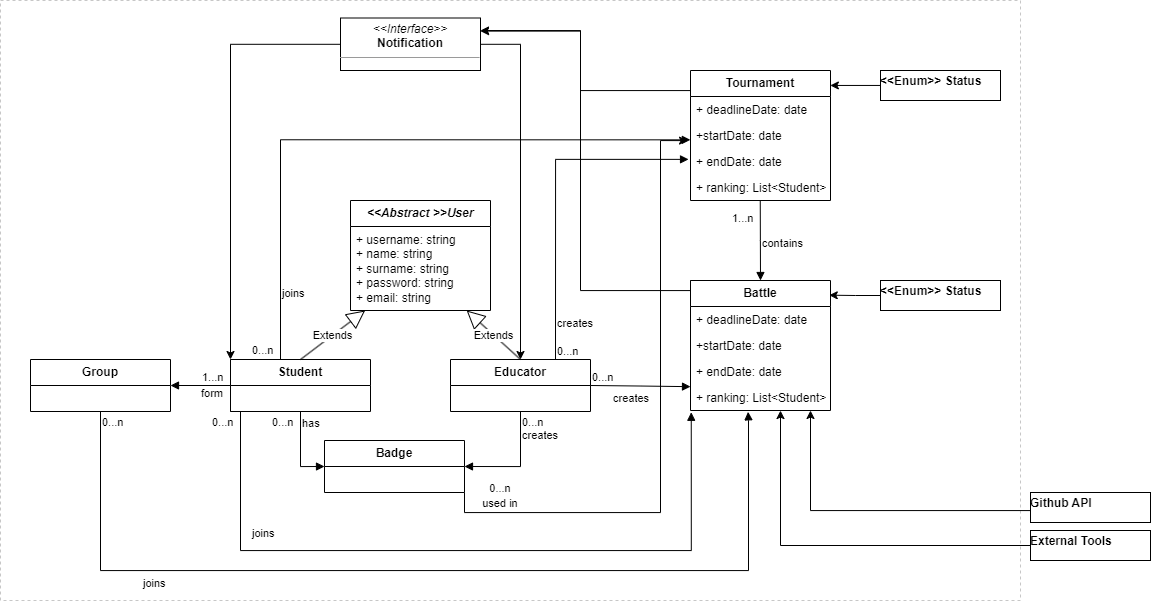
\includegraphics[width=0.9\linewidth]{UML_v2.png}
        \caption{High level Class Diagram.}
        \label{fig:UML}%
    \end{center}
\end{figure}

TODO
Fix class diagram and add a brief description


\subsection{State diagrams}
\label{subsec:state_diagrams}%
In this section are presented the State Diagrams of the S\&C system representing possible operations that a user can perform.
TODO

\paragraph{Name}
Brief description

\begin{figure}[H]
    \begin{center}
        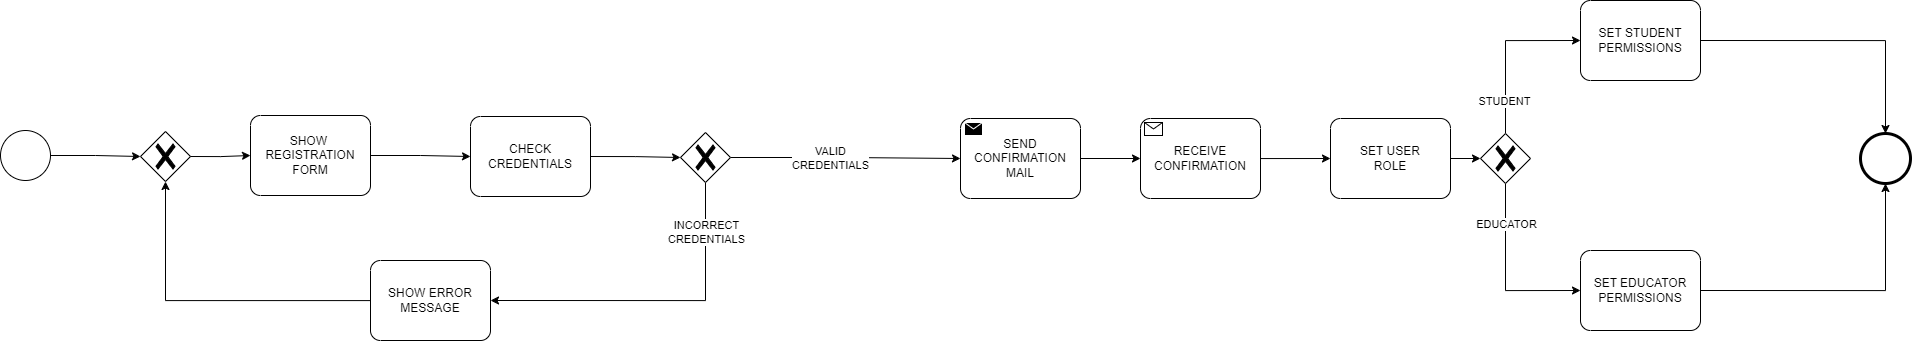
\includegraphics[width=1\linewidth]{StateDiagrams/signup.png}
        \caption{Figure}
        \label{fig:signup_sd}%
    \end{center}
\end{figure}

Repeat

\section{Product functions}
\label{sec:product_functions}%
Here are listed a summary of the main functions of the S\&C system:\\\\
\textbf{ Sign-up:} The User submits his name, surname, email address and a new password. A confirmation mail is required to complete the process.\\\\
\textbf{ Login:} The User sign in after typing his email and password in the login form. \\\\  
\textbf{ Update CV:} A ST can update their data after creating a new account, including experience, skills, attitude and the resume .\\\\
\textbf{ Publish an internship:} A CP can publish an internship proposal through  the "create new internship" section.\\\\
\textbf{ Search for an internship:} A ST can look for an internship by keyword search or by setting some predefined filters, even both simultaneously.\\\\
\textbf{ Apply for an internship:} A ST can apply for an internship by clicking on the "Apply" button on an internship post.\\\\
\textbf{ Ask for a ST application: } A CP can send a notification of interest to a student from the list of recommendations provided by the system.\\\\
\textbf{ Reviewing an apply request:} A company can decide whether to accept or reject a student's application from the application section or after receiving a notification via the inbox.\\\\
\textbf{ Create task for interviews:}  A CP can prepare tasks or questionnaires to evaluate candidates through the system's interview management section. These tasks may include technical challenges, situational assessments, or other relevant exercises, which are assigned to candidates. Once the tasks are completed and reviewed, the CP can schedule further interviews directly through the system, specifying the date, time, and format, and notifying candidates. \\\\
\textbf{ Solve tasks and questionnaires:} A ST can access and complete the tasks or questionnaires assigned by a CP through their profile. After submission, the system automatically records their responses and notifies the CP about the completion, allowing them to evaluate the candidate's performance.\\\\
\textbf{ Finalize selections :} After reviewing completed tasks and conducting interviews, a CP can finalize their selections for an internship position. This includes marking the selected students and notifying them through the system, while also sending updates to unselected candidates.
\\\\
\textbf{ Logout:} A User session will be closed if the User clicks on "Logout" button. Next time the User opens S\&C he will need to log in again.

\section{User characteristic}
\label{sec:User_characteristic}%
TODO

\section{Assumptions, dependencies and constraints}
\label{sec:assumptions_dependencies_constraints}%

\subsection{Domain assumptions}
\label{subsec:domain_assumptions}%
TODO
\newcounter{da}
\setcounter{da}{1}
\newcommand{\cda}{\theda\stepcounter{da}}
\begin{center}
    \begin{longtable}{ |l|p{0.9\linewidth}| }
        \hline
        \textbf{ID} & \textbf{Description} \\
        \hline
        DA\cda      & The EDs need to have a valid eMail address. \\
        \hline
        DA\cda      & The STs need to have a valid eMail address. \\
        \hline
        DA\cda      & The EDs need to have a device and a reliable internet connection. \\
        \hline
        DA\cda      & The STs need to have a device and a reliable internet connection. \\
        \hline
        DA\cda      & The EDs need to have a GitHub account. \\
        \hline
        DA\cda      & The STs need to have a GitHub account. \\
        \hline
        DA\cda      & STs need to know how to fork a GitHub Repository. \\
        \hline
        DA\cda      & STs need to know how to push their code on GitHub. \\
        \hline
        DA\cda      & CKB needs to communicate with GH through its API. \\
        \hline
        DA\cda      & CKB needs to communicate with the external Static Analysis Tools in order to compute the scores. \\
        \hline
        DA\cda      & CKB needs to communicate correctly with the eMail system. \\
        \hline
        \caption{Domain assumptions.}
        \label{tab:domainassmptn_tab}%
    \end{longtable}
\end{center}


    \chapter{Specific Requirements}
    \label{ch:specific_requirements}%
    \section{External interface requirements}
\label{sec:external_interface_requirements}%

\subsection{User interfaces}
\label{subsec:User_interfaces}%
The S\&C system will be a web app accessible by different devices and form factors, with a responsive UI. The UI will be different based on the type of user, reflecting the different functionalities they need. Every user will need to insert their credentials to have access to the platform and there will be a mechanism to recover them in case of a loss. The UI will comply with accessibility standards to ensure usability for all users, including those with disabilities.

\subsection{Hardware interfaces}
\label{subsec:hardware_interfaces}%
Our platform is a web app, as a consequence, it does not require any specific hardware
interface. Users only need a device with a browser to access the website and an internet connection. Latest versions of browsers are suggested to ensure compatibility and optimal performance. The user is free to choose his device but accessing the web app from a desktop form factor is strongly recommended for the best user experience.


\subsection{Software interfaces}
\label{subsec:software_interfaces}%
No specific software interfaces are needed. However, a mailing system to send confirmation emails will be used to the users during the registration process. In the future, integrations with university and company tools will be possible to enhance interoperability.

\subsection{Communication interfaces}
\label{subsec:communication_interfaces}%
The communication interfaces needed by the system include the HTTPS protocol for secure data transfer between the client and server. SSL/TLS certificates will ensure encrypted communication to protect user credentials and sensitive information.

\section{Functional requirements}
\label{sec:functional_requirements}%

\subsection{Requirements}
\label{subsec:requirements3}%
\newcounter{req}
\setcounter{req}{1}
\newcommand{\creq}{\thereq\stepcounter{req}}
\begin{center}
    \begin{longtable}{|l|p{0.9\linewidth}|}
        \hline
        \textbf{ID} & \textbf{Description}\\
        \hline
        R\creq & {The system allows STs to register by providing personal information, email, and a password.}\\
        \hline
        R\creq & {The system shall allow Users to log in using their credentials.}\\
        \hline
        R\creq & {The system shall allow STs to edit their profiles, including personal details and contact information.}\\
        \hline
        R\creq & {The system shall enforce role-based access control to restrict access to specific functionalities based on the user type (ST, CP, UV).}\\
        \hline
        R\creq & {The system shall allow CPs to post new internship opportunities, including position details, required skills, duration, and compensation.}\\
        \hline
        R\creq & {The system shall allow STs to apply for internships by submitting a CV and optional cover letter.}\\
        \hline
        R\creq & {The system shall notify CPs when STs apply to an internship.}\\
        \hline
        R\creq & {The system shall allow CPs to review applications and schedule interviews with STs.}\\
        \hline
        R\creq & {The system shall allow CPs to submit questionnaires to STs.}\\
        \hline
        R\creq & {The system shall allow CPs to accept or reject applications and notify STs of the decision.}\\
        \hline
        R\creq & {The system shall allow UVs to manage their students and monitor their activity.}\\
        \hline
        R\creq & {The system shall send notifications to users for events such as application submissions, approvals, or rejections.}\\
        \hline
        R\creq & {The system shall allow CPs to track the progress of STs during the internship and provide regular feedback.}\\
        \hline
        R\creq & {The system shall allow CPs to evaluate the performance of STs at the end of the internship.}\\
        \hline
        R\creq & {The system shall allow UVs to review the feedback and evaluation provided by both CPs and STs.}\\
        \hline
        R\creq & {The system shall allow STs to search for internships using keywords, filters, or location.}\\
        \hline
        R\creq & {The system shall recommend internships to STs based on their skills, preferences, and past applications.}\\
        \hline
        R\creq & {The system shall recommend STs to CPs for specific internships based on their skills, preferences, and past applications.}\\
        \hline
        R\creq & {The system shall allow CPs to search for suitable STs based on their skills, academic background, and CVs.}\\
        \hline
        R\creq & {The system shall maintain a database of all internships, applications, and evaluations.}\\
        \hline
        \caption{Requirements.}
        \label{tab: requirements}%
    \end{longtable}
\end{center}

\subsection{Use case diagrams}
\label{subsec:use_case_diagrams}%

\begin{figure}[H]
    \begin{center}
        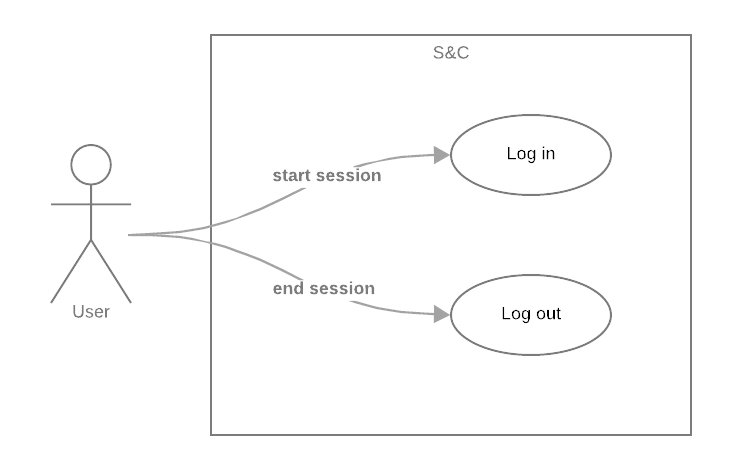
\includegraphics[width=0.8\linewidth]{UseCaseDiagrams/User.png}
        \caption{Use Cases Diagram for all users.} 
        \label{fig:UserUC}%
    \end{center}
\end{figure}

\begin{figure}[H]
    \begin{center}
        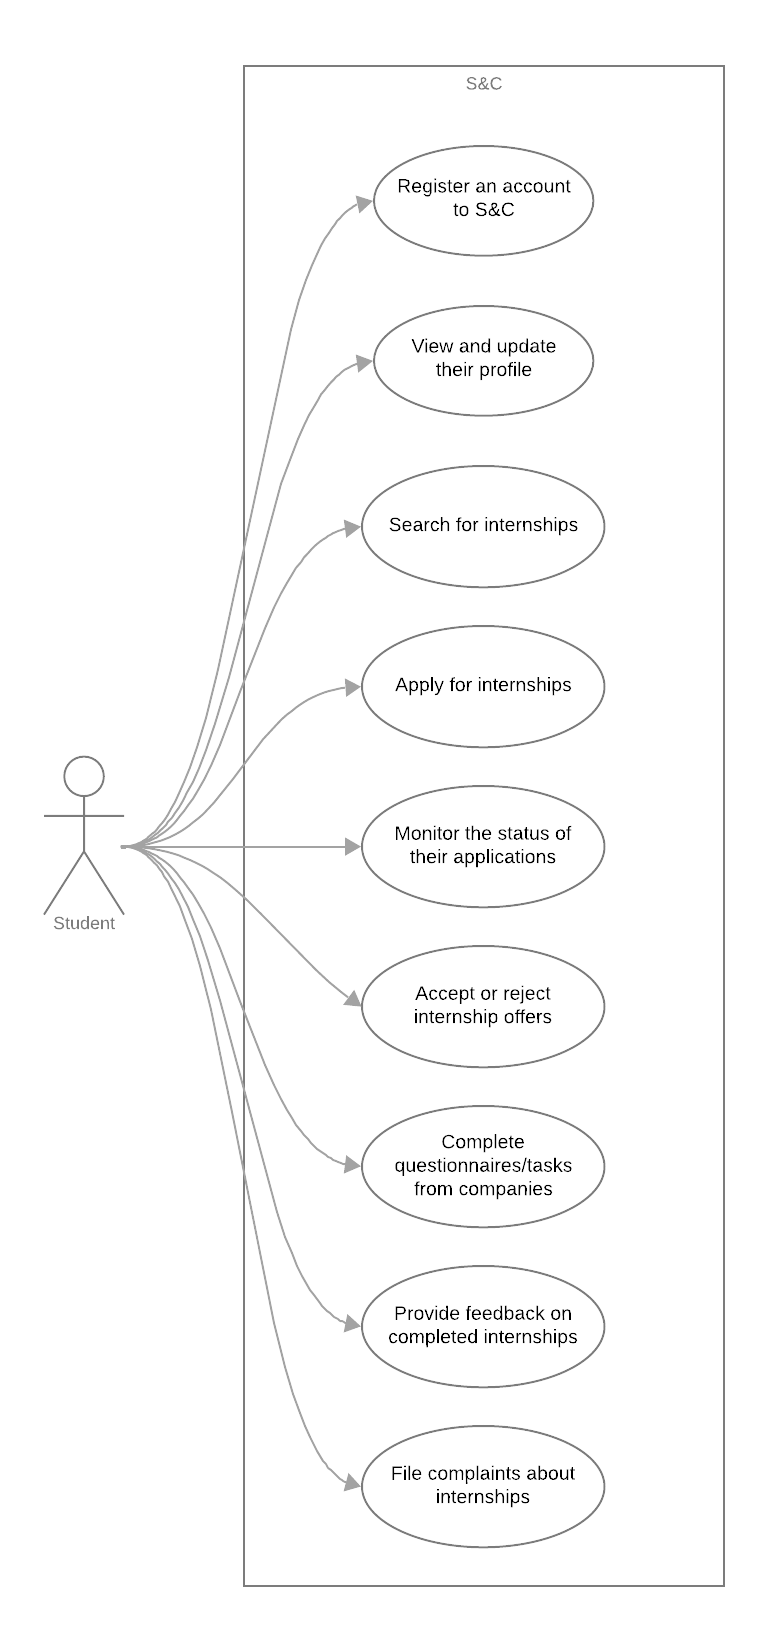
\includegraphics[width=0.6\linewidth]{UseCaseDiagrams/Student.png}
        \caption{Use Cases Diagram for students.} 
        \label{fig:StudentUC}%
    \end{center}
\end{figure}

\begin{figure}[H]
    \begin{center}
        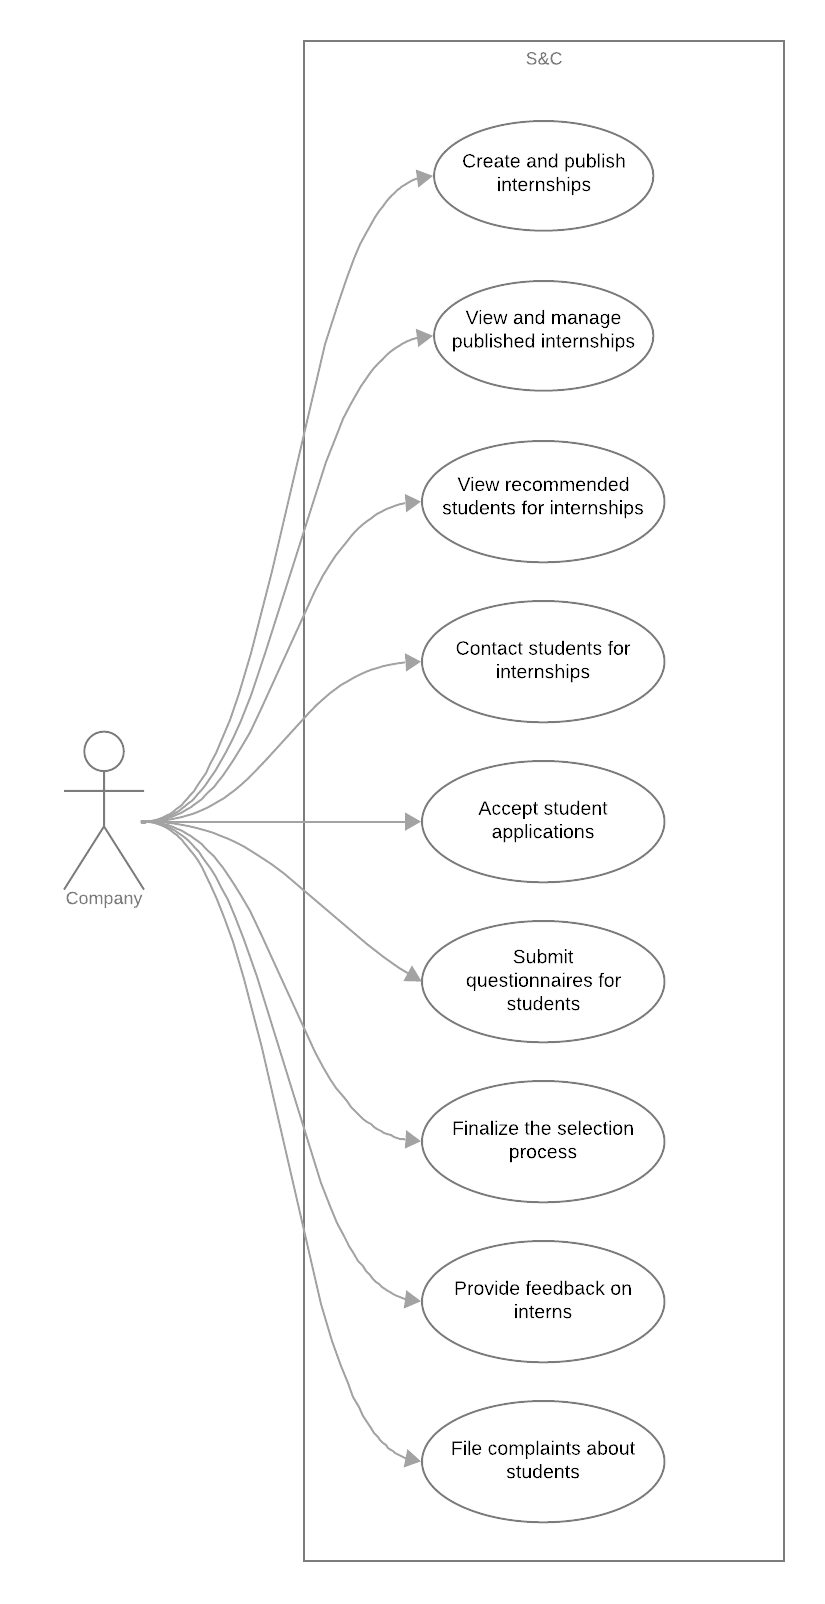
\includegraphics[width=0.8\linewidth]{UseCaseDiagrams/Company.png}
        \caption{Use Cases Diagram for companies.} 
        \label{fig:CompanyUC}%
    \end{center}
\end{figure}

\begin{figure}[H]
    \begin{center}
        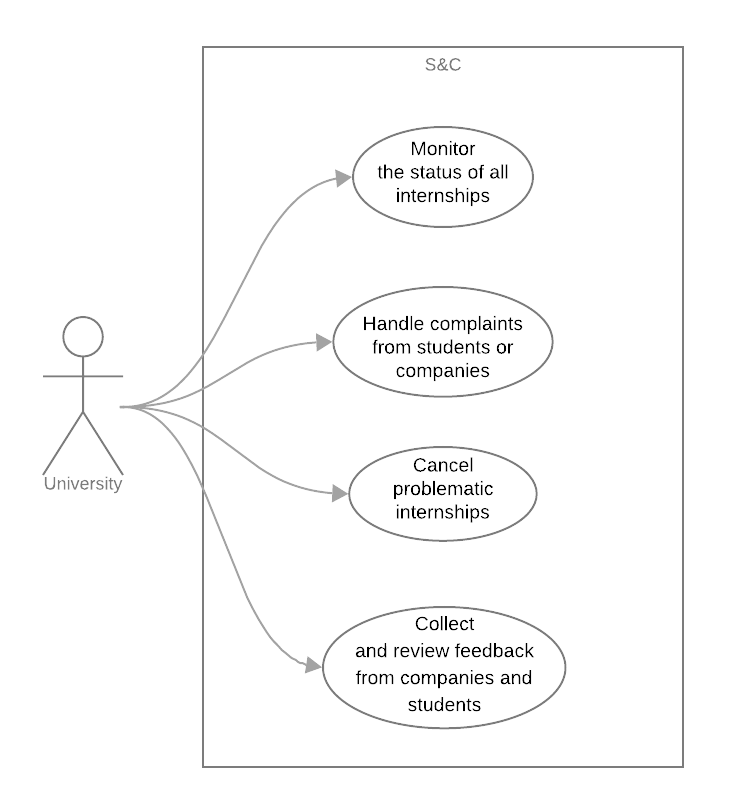
\includegraphics[width=0.6\linewidth]{UseCaseDiagrams/University.png}
        \caption{Use Cases Diagram for universities.} 
        \label{fig:UniversityUC}%
    \end{center}
\end{figure}

\begin{figure}[H]
    \begin{center}
        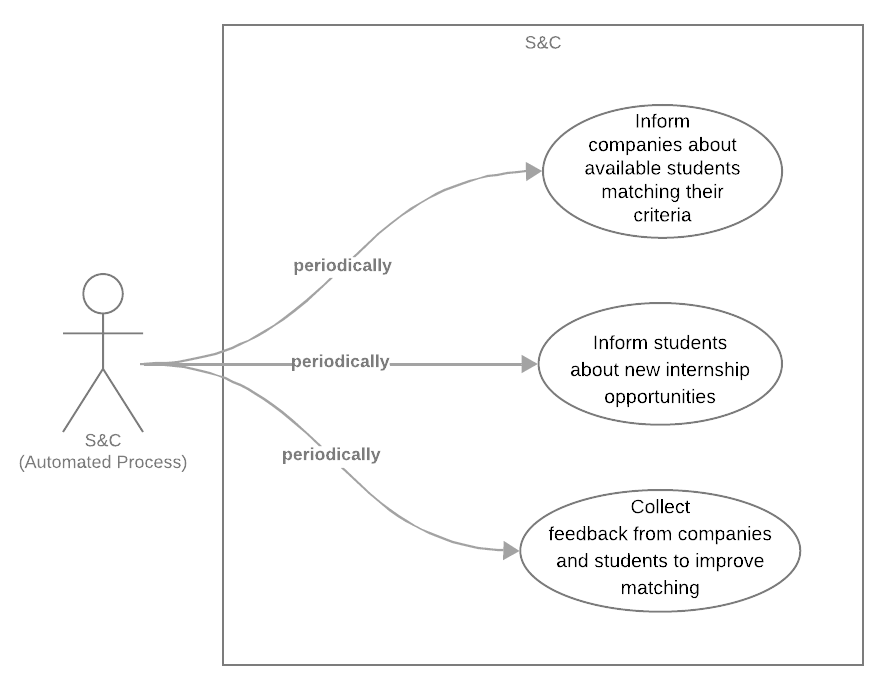
\includegraphics[width=0.6\linewidth]{UseCaseDiagrams/SeC.png}
        \caption{Use Cases Diagram for S\&C.} 
        \label{fig:SeCUC}%
    \end{center}
\end{figure}

\newpage
\subsection{Use cases}
\label{subsec: use_cases}%
\newcounter{uc}
\setcounter{uc}{1}
\newcommand{\cuc}{\theuc\stepcounter{uc}}
This section explains the main use cases and how they work. It includes a table for each use case that shows the starting conditions, steps involved, ending conditions, and any exceptions. There's also a sequence diagram that illustrates the messages exchanged between different entities and the functions that are called. \\

\subsubsection*{UC\cuc . Log in to the system}
\begin{center}
    \begin{longtable}{|l|p{0.75\linewidth}|}
        \hline
        \textbf{Actor}            & Student (ST), Company (CP), University (UV) \\
        \hline
        \textbf{Entry conditions} & The user has valid credentials (email and password) and access to S\&C's login page. \\
        \hline
        \textbf{Event Flow}       & 1 - The user navigates to the login page. \\
                                  & 2 - The user inputs their email and password. \\
                                  & 3 - S\&C validates the credentials. \\
                                  & 4 - The user is redirected to their respective dashboard. \\
        \hline
        \textbf{Exit condition}   & The user is logged into S\&C and has access to their dashboard. \\       
        \hline
        \textbf{Exceptions}       & - Incorrect email or password: The system displays an error message. \\
                                  & - System unavailable: S\&C informs the user and retries later. \\
        \hline
        \caption{Log in to the system}
        \label{tab:login_usecase}
    \end{longtable}
\end{center}

\begin{figure}[H]
    \begin{center}
        \includesvg[width=\textwidth]{SequenceDiagrams/Login.svg}
        \caption{Log in to the system sequence diagram.}
        \label{fig:login_seqd}%
    \end{center}
\end{figure}

\subsubsection*{UC\cuc . Log out from the system}
\begin{center}
    \begin{longtable}{|l|p{0.75\linewidth}|}
        \hline
        \textbf{Actor}            & Student (ST), Company (CP), University (UV) \\
        \hline
        \textbf{Entry conditions} & The user is logged into S\&C and has access to their dashboard. \\
        \hline
        \textbf{Event Flow}       & 1 - The user clicks the "Log Out" button. \\
                                  & 2 - S\&C invalidates the user's session. \\
                                  & 3 - S\&C redirects the user to the login page. \\
        \hline
        \textbf{Exit condition}   & The user is logged out of S\&C and redirected to the login page. \\       
        \hline
        \textbf{Exceptions}       & - System unavailable: S\&C informs the user and retries later. \\
        \hline
        \caption{Log out from the system}
        \label{tab:logout_usecase}
    \end{longtable}
\end{center}

\begin{figure}[H]
    \begin{center}
        \includesvg[width=0.8\textwidth]{SequenceDiagrams/Logout.svg}
        \caption{Log out from the system sequence diagram.}
        \label{fig:logout_seqd}%
    \end{center}
\end{figure}

\subsubsection*{UC\cuc . Register an account to S\&C}
TODO

\subsubsection*{UC\cuc . View and update their profile}
\begin{center}
    \begin{longtable}{|l|p{0.75\linewidth}|}
        \hline
        \textbf{Actor}            & Student (ST) \\
        \hline
        \textbf{Entry conditions} & The student is logged into S\&C. \\
        \hline
        \textbf{Event Flow}       & 1 - The user navigates to the profile section. \\
        & 2 - The user views their profile details. \\
        & 3 - The user updates specific fields (e.g., contact info, skills, CV). \\
        & 4 - S\&C validates the changes. \\
        & 5 - S\&C saves the updated profile. \\
        \hline
        \textbf{Exit condition}   & The user's profile is updated and saved successfully. \\       
        \hline
        \textbf{Exceptions}       & - Invalid data: S\&C prompts the user to correct the information. \\
                                  & - System unavailable: S\&C informs the user and retries later. \\
        \hline
        \caption{View and update their profile}
        \label{tab:view_update_profile_usecase}
    \end{longtable}
\end{center}

\begin{figure}[H]
    \begin{center}
        \includesvg[width=0.8\textwidth]{SequenceDiagrams/View_And_Update.svg}
        \caption{View and update profile sequence diagram.}
        \label{fig:view_update_profile_seqd}%
    \end{center}
\end{figure}

\subsubsection*{UC\cuc . Search for internships}
\begin{center}
    \begin{longtable}{|l|p{0.75\linewidth}|}
        \hline
        \textbf{Actor}            & Student (ST) \\
        \hline
        \textbf{Entry conditions} & The user is logged into S\&C. \\
        \hline
        \textbf{Event Flow}       & 1 - The user navigates to the internships section. \\
        & 2 - The user searches (e.g. by keywords, location, filters). \\
        & 3 - S\&C processes the search and retrieves results. \\
        & 4 - The user views the list of available internships. \\
        \hline
        \textbf{Exit condition}   & The user views relevant internship opportunities. \\       
        \hline
        \textbf{Exceptions}       & - No results: S\&C informs the user that no internships match the criteria. \\
                                  & - System unavailable: S\&C informs the user and retries later. \\
        \hline
        \caption{Search for internships}
        \label{tab:search_internships_usecase}
    \end{longtable}
\end{center}

\begin{figure}[H]
    \begin{center}
        \includesvg[width=0.8\textwidth]{SequenceDiagrams/Search_Internships.svg}
        \caption{Search for internships sequence diagram.}
        \label{fig:search_internships_seqd}%
    \end{center}
\end{figure}

\subsubsection*{UC\cuc . Apply for an internship}
\begin{center}
    \begin{longtable}{|l|p{0.75\linewidth}|}
        \hline
        \textbf{Actor}            & Student (ST) \\
        \hline
        \textbf{Entry conditions} & The user is logged into S\&C and has selected an internship. \\
        \hline
        \textbf{Event Flow}       & 1 - The user navigates to the internship details page. \\
        & 2 - The user clicks the "Apply" button. \\
        & 3 - S\&C validates the user's eligibility. \\
        & 4 - S\&C submits the application. \\
        & 5 - S\&C confirms the application to the user. \\
        \hline
        \textbf{Exit condition}   & The user's application is successfully submitted. \\       
        \hline
        \textbf{Exceptions}       & - Not eligible: S\&C notifies the user with the reason for ineligibility (e.g. does not have the necessary skills). \\
                                  & - System unavailable: S\&C informs the user and retries later. \\
        \hline
        \caption{Apply for an internship}
        \label{tab:apply_internship_usecase}
    \end{longtable}
\end{center}

\begin{figure}[H]
    \begin{center}
        \includesvg[width=0.8\textwidth]{SequenceDiagrams/Apply_Internship.svg}
        \caption{Apply for an internship sequence diagram.}
        \label{fig:apply_internship_seqd}%
    \end{center}
\end{figure}

\subsubsection*{UC\cuc . Monitor the status of their applications}
\begin{center}
    \begin{longtable}{|l|p{0.75\linewidth}|}
        \hline
        \textbf{Actor}            & Student (ST) \\
        \hline
        \textbf{Entry conditions} & The user is logged into S\&C and has submitted at least one application. \\
        \hline
        \textbf{Event Flow}       & 1 - The user navigates to the "My Applications" section. \\
        & 2 - S\&C retrieves the status of all submitted applications. \\
        & 3 - The user views the list of applications and their statuses. \\
        \hline
        \textbf{Exit condition}   & The user views the status of their applications. \\       
        \hline
        \textbf{Exceptions}       & - No applications: S\&C informs the user that no applications have been submitted. \\
                                  & - System unavailable: S\&C informs the user and retries later. \\
        \hline
        \caption{Monitor the status of their applications}
        \label{tab:monitor_status_applications_usecase}
    \end{longtable}
\end{center}

\begin{figure}[H]
    \begin{center}
        \includesvg[width=1\textwidth]{SequenceDiagrams/Monitor_Status.svg}
        \caption{Monitor the status of their applications sequence diagram.}
        \label{fig:monitor_status_seqd}%
    \end{center}
\end{figure}

\subsubsection*{UC\cuc . Accept or reject internship offers}
\begin{center}
    \begin{longtable}{|l|p{0.75\linewidth}|}
        \hline
        \textbf{Actor}            & Student (ST) \\
        \hline
        \textbf{Entry conditions} & The user is logged into S\&C and has received at least one internship offer. \\
        \hline
        \textbf{Event Flow}       & 1 - The user navigates to the "Offers" section. \\
        & 2 - S\&C retrieves the list of received offers. \\
        & 3 - The user selects an offer to review. \\
        & 4 - The user chooses to accept or reject the offer. \\
        & 5 - S\&C updates the offer status. \\
        \hline
        \textbf{Exit condition}   & The offer status is updated as accepted or rejected. \\       
        \hline
        \textbf{Exceptions}       & - Offer expired: S\&C notifies the user. \\
                                  & - System unavailable: S\&C informs the user and retries later. \\
        \hline
        \caption{Accept or reject internship offers}
        \label{tab:accept_reject_offers_usecase}
    \end{longtable}
\end{center}

\begin{figure}[H]
    \begin{center}
        \includesvg[width=0.8\textwidth]{SequenceDiagrams/Accept_Reject_Offers.svg}
        \caption{Accept or reject internship offers sequence diagram.}
        \label{fig:accept_reject_offers_seqd}%
    \end{center}
\end{figure}

\subsubsection*{UC\cuc . Complete questionnaires from companies}
TODO

\subsubsection*{UC\cuc . Provide feedback on completed internships}
\begin{center}
    \begin{longtable}{|l|p{0.75\linewidth}|}
        \hline
        \textbf{Actor}            & Student (ST) \\
        \hline
        \textbf{Entry conditions} & The user is logged into S\&C and has completed at least one internship. \\
        \hline
        \textbf{Event Flow}       & 1 - The user navigates to the "Completed Internships" section. \\
        & 2 - S\&C retrieves the list of completed internships. \\
        & 3 - The user selects an internship to provide feedback on. \\
        & 4 - The user fills out the feedback form. \\
        & 5 - S\&C saves the user's feedback. \\
        \hline
        \textbf{Exit condition}   & Feedback for the internship is successfully submitted. \\       
        \hline
        \textbf{Exceptions}       & - System unavailable: S\&C informs the user and retries later. \\
        \hline
        \caption{Provide feedback on completed internships}
        \label{tab:provide_feedback_usecase}
    \end{longtable}
\end{center}

\begin{figure}[H]
    \begin{center}
        \includesvg[width=1\textwidth]{SequenceDiagrams/Provide_Feedback.svg}
        \caption{Provide feedback on completed internships sequence diagram.}
        \label{fig:provide_feedback_seqd}%
    \end{center}
\end{figure}

\subsubsection*{UC\cuc . File complaints about internships}
\begin{center}
    \begin{longtable}{|l|p{0.75\linewidth}|}
        \hline
        \textbf{Actor}            & Student (ST) \\
        \hline
        \textbf{Entry conditions} & The user is logged into S\&C and has encountered an issue with an internship. \\
        \hline
        \textbf{Event Flow}       & 1 - The user navigates to the "Complaints" section. \\
        & 2 - S\&C provides the complaint form. \\
        & 3 - The user fills out the complaint form, describing the issue. \\
        & 4 - The user submits the complaint. \\
        & 5 - S\&C saves and forwards the complaint to the relevant parties. \\
        \hline
        \textbf{Exit condition}   & The complaint is successfully filed and acknowledged by S\&C. \\       
        \hline
        \textbf{Exceptions}       & - System unavailable: S\&C informs the user and retries later. \\
        \hline
        \caption{File complaints about internships}
        \label{tab:file_complaints_usecase}
    \end{longtable}
\end{center}

\begin{figure}[H]
    \begin{center}
        \includesvg[width=1\textwidth]{SequenceDiagrams/File_Complaints.svg}
        \caption{File complaints about internships sequence diagram.}
        \label{fig:file_complaints_seqd}%
    \end{center}
\end{figure}

\subsubsection*{UC\cuc . Create and publish internships}
TODO

\subsubsection*{UC\cuc . View and manage published internships}
TODO

\subsubsection*{UC\cuc . View recommended students for internships}
TODO

\subsubsection*{UC\cuc . Contact students for internships}
TODO

\subsubsection*{UC\cuc . Accept student applications}
TODO

\subsubsection*{UC\cuc . Submit questionnaires for students}
TODO

\subsubsection*{UC\cuc . Finalize the selection process}
TODO

\subsubsection*{UC\cuc . Provide feedback on interns}
TODO

\subsubsection*{UC\cuc . File complaints about students}
TODO

\subsubsection*{UC\cuc . Monitor the status of all internships}
TODO

\subsubsection*{UC\cuc . Handle complaints from students or companies}
TODO

\subsubsection*{UC\cuc . Cancel problematic internships}
TODO

\subsubsection*{UC\cuc . Collect and review feedback from companies and students}
TODO

\subsubsection*{UC\cuc . Inform companies about available students matching their criteria}
TODO

\subsubsection*{UC\cuc . Inform students about new internship opportunities}
TODO

\newpage

\subsection{Requirement mapping}
\label{subsec:requirement_mapping}%
\textbf{G1 - Allow companies to post their internship opportunities.}
\begin{itemize}
    \item R2: The system shall allow Users to log in using their credentials.
    \item R4: The system shall enforce role-based access control to restrict access to specific functionalities based on the user type (ST, CP, UV).
    \item R5: The system shall allow CPs to post new internship opportunities, including position details, required skills, duration, and compensation.
    \item R20: The system shall maintain a database of all internships, applications, and evaluations.
\end{itemize}

\vspace{1.5cm}
\textbf{G2 - Allow students to search for available internships.}
\begin{itemize}
    \item R1: The system allows STs to register by providing personal information, email, and a password.
    \item R2: The system shall allow Users to log in using their credentials.
    \item R3: The system shall allow STs to edit their profiles, including personal details and contact information.
    \item R16: The system shall allow STs to search for internships using keywords, filters, or location.
    \item R17: The system shall recommend internships to STs based on their skills, preferences, and past applications.
\end{itemize}

\vspace{1.5cm}
\textbf{G3 - Notify students when an internship that might be of interest to them is posted.}
\begin{itemize}
    \item R12: The system shall send notifications to users for events such as application submissions, approvals, or rejections.
    \item R17: The system shall recommend internships to STs based on their skills, preferences, and past applications.
\end{itemize}

\vspace{1.5cm}
\textbf{G4 - Notify companies when a student matching their needs becomes available.}
\begin{itemize}
    \item R6: The system shall allow STs to apply for internships by submitting a CV and optional cover letter.
    \item R7: The system shall notify CPs when STs apply to an internship.
    \item R18: The system shall recommend STs to CPs for specific internships based on their skills, preferences, and past applications.
\end{itemize}

\vspace{1.5cm}
\textbf{G5 - Provide tools for both companies and students to manage the selection process.}
\begin{itemize}
    \item R2: The system shall allow Users to log in using their credentials.
    \item R8: The system shall allow CPs to review applications and schedule interviews with STs.
    \item R9: The system shall allow CPs to submit questionnaires to STs.
    \item R10: The system shall allow CPs to accept or reject applications and notify STs of the decision.
    \item R19: The system shall allow CPs to search for suitable STs based on their skills, academic background, and CVs.
\end{itemize}

\vspace{1.5cm}
\textbf{G6 - Collect feedback from students and companies to improve the matchmaking process.}
\begin{itemize}
    \item R2: The system shall allow Users to log in using their credentials.
    \item R13: The system shall allow CPs to track the progress of STs during the internship and provide regular feedback.
    \item R14: The system shall allow CPs to evaluate the performance of STs at the end of the internship.
    \item R15: The system shall allow UVs to review the feedback and evaluation provided by both CPs and STs.
\end{itemize}

\vspace{1.5cm}
\textbf{G7 - Provide suggestions for companies to improve internship descriptions and for students to improve their resumes.}
\begin{itemize}
    \item R4: The system shall enforce role-based access control to restrict access to specific functionalities based on the user type (ST, CP, UV).
    \item R17: The system shall recommend internships to STs based on their skills, preferences, and past applications.
    \item R18: The system shall recommend STs to CPs for specific internships based on their skills, preferences, and past applications.
\end{itemize}

\vspace{1.5cm}
\textbf{G8 - Allow all parties to monitor the status of the matchmaking process and the assigned internship.}
\begin{itemize}
    \item R2: The system shall allow Users to log in using their credentials.
    \item R13: The system shall allow CPs to track the progress of STs during the internship and provide regular feedback.
    \item R20: The system shall maintain a database of all internships, applications, and evaluations.
\end{itemize}

\vspace{1.5cm}
\textbf{G9 - Allow universities to monitor internships and handle any problems.}
\begin{itemize}
    \item R2: The system shall allow Users to log in using their credentials.
    \item R11: The system shall allow UVs to manage their students and monitor their activity.
    \item R12: The system shall send notifications to users for events such as application submissions, approvals, or rejections.
    \item R15: The system shall allow UVs to review the feedback and evaluation provided by both CPs and STs.
\end{itemize}

\vspace{2cm}
\newcounter{rtt}
\setcounter{rtt}{1}
\newcommand{\crt} {\thertt\stepcounter{rtt}}
\begin{center}
     \begin{longtable}{|l|c|c|c|c|c|c|c|c|c|}
    \hline
    \textbf{Requirements} & \textbf{G1} & \textbf{G2} & \textbf{G3} & \textbf{G4} & \textbf{G5} & \textbf{G6} & \textbf{G7} & \textbf{G8} & \textbf{G9}\\ \hline
    R1 &  & \checkmark  &  &  &  &  &  &  &  \\ \hline
    R2 & \checkmark & \checkmark & & & \checkmark & \checkmark & & \checkmark & \checkmark \\ \hline
    R3 &  & \checkmark &  &  &  &  &  &  &  \\ \hline
    R4 & \checkmark &  &  &  &  &  & \checkmark &  &  \\ \hline
    R5 & \checkmark &  &  &  &  &  &  &  &  \\ \hline
    R6 &  &  &  & \checkmark &  &  &  &  &  \\ \hline
    R7 &  &  &  & \checkmark &  &  &  &  &  \\ \hline
    R8 &  &  &  &  & \checkmark &  &  &  &  \\ \hline
    R9 &  &  &  &  & \checkmark &  &  &  &  \\ \hline
    R10 &  &  &  &  & \checkmark &  &  &  &  \\ \hline
    R11 &  &  &  &  &  &  &  &  & \checkmark \\ \hline
    R12 &  &  & \checkmark &  &  &  &  &  & \checkmark \\ \hline
    R13 &  &  &  &  &  & \checkmark &  & \checkmark &  \\ \hline
    R14 &  &  &  &  &  & \checkmark &  &  &  \\ \hline
    R15 &  &  &  &  &  & \checkmark &  &  & \checkmark \\ \hline
    R16 &  & \checkmark &  &  &  &  &  &  &  \\ \hline
    R17 &  & \checkmark & \checkmark &  &  &  & \checkmark &  &  \\ \hline
    R18 &  &  &  & \checkmark &  &  & \checkmark &  &  \\ \hline
    R19 &  &  &  &  & \checkmark &  &  &  &  \\ \hline
    R20 & \checkmark &  &  &  &  &  &  & \checkmark &  \\ \hline
\caption{Traceability Matrix for Goals and Requirements}
\label{tab:traceability}
\end{longtable}
\end{center}

\section{Performance requirements}
\label{sec:performance_requirements}%

\paragraph{Number of Concurrent Users:}
The S\&C system is expected to handle a significant number of concurrent users, based on research from similar platforms. The system architecture will be designed to scale dynamically to ensure consistent performance under heavy loads. Load testing will be conducted during development to verify this capacity.

\paragraph{Data Storage and Management:}
The system must efficiently handle large volumes of data, including:
\begin{itemize}
    \item Personal information of Students (ST) and Companies (CP).
    \item Records of all Internship Listings, Applications, and Interactions between users.
    \item Historical data for old internship offers. This information will remain stored indefinitely to allow CPs to review their previous postings and applicants.
\end{itemize}
To ensure scalability, a database management system with high throughput will be used. Additionally, data archiving strategies will be implemented to optimize storage for historical data without affecting performance.

\paragraph{Response Time:}
Actions executed directly by the S\&C system must have a response time of less than 500 milliseconds in normal conditions. Operations involving external services such as email systems may experience delays depending on the response times of those services. In case of a slow internet connection on the user's side, performance might degrade..

\section{Design constraints}
\label{sec:design_constraints}%

\subsection{Standard compliance}
\label{subsec:standard compliance}%%
The system must be compliant with the following standards and regulations:
\begin{itemize}
    \item EU's GDPR (General Data Protection Regulation), a set of regulations that is designed in order to protect the personal data, the privacy and security of the EU's citizens.
    \item WCAG (Web Content Accessibility Guidelines): The user interface will follow WCAG 2.1 Level AA guidelines to ensure accessibility for users with disabilities. This includes providing text alternatives for non-text content, keyboard navigation support, and ensuring sufficient contrast in the UI design.
\end{itemize}

\subsection{Hardware limitations}
\label{subsec:hardware_limitations}%
The platform is designed as a web application and does not require specific hardware. The users must have a device with a modern web browser and a reliable internet connection with a minimum recommended speed of 2 Mbps to ensure a smooth experience.

\section{Software system attributes}
\label{sec:software_system_attributes}%

\subsection{Reliability}
\label{subsec:reliability}%
The system has to be reliable because it will have to run continuously for a long period
of time. To ensure this feature the platform must have:
\begin{itemize}
    \item Some sort of replication and consistency policy to avoid system crash.
    \item Offline backups of the system in multiple locations to recover information after data loss or catastrophic failures.
    \item A monitoring system that alerts administrators in case of problems.
\end{itemize}

\subsection{Availability}
\label{subsec:availability}%
The most important attribute that the system has to provide is the availability. The
system should have an availability of 99\% to not interfere with users’ activities. To achieve this:
\begin{itemize}
    \item Replication policies must be implemented and a single point of failure should be avoided.
    \item Maintenance should be scheduled during low traffic periods (e.g., late-night) and notify users in advance.
    \item The recommendation algorithm should be optimized to run primarily during low-load hours, minimizing the impact on system performance during peak usage.
\end{itemize}

\subsection{Security}
\label{subsec:security}%
To protect user data and system integrity. The system must implement:
\begin{itemize}
    \item Authentication and authorization mechanisms, ensuring that only verified users can access the platform and perform actions based on their roles.
    \item Encryption for all sensitive data and communications between the client and server.
    \item Protection against common web vulnerabilities.
    \item Logging and monitoring of suspicious activities, such as repeated failed login attempts or unauthorized access attempts.
\end{itemize}

\subsection{Maintainability}
\label{subsec:maintainability}%
To ensure maintainability of the system the following actions are required:
\begin{itemize}
    \item Fllow modular and reusable design principles, ensuring that individual components can be updated or replaced without affecting the entire system.
    \item The code has to be well documented.
    \item A testing routine has to be provided and it has to cover at least 75\% of the entire code excluding the UI code.
\end{itemize}

\subsection{Portability}
\label{subsec:portability}%
The system should be portable, ensuring access across different platforms and environments.
\begin{itemize}
    \item Client-side the platform must be compatible with modern web browsers on both desktop and mobile devices.
    \item Server-side the backend should be deployable on multiple hosting environments, such as on-premises servers or cloud platforms without significant modifications. To ease this, use of containerization technologies is suggested.
\end{itemize}


    \chapter{Formal Analysis Using Alloy}
    \label{ch:formal_analysis_using_alloy}%
    Here is an alloy specification of the system described in the RASD: 
\vspace{2cm}
\lstinputlisting[language=alloy]{Alloy/SeC.als}
\newpage

\begin{figure}[H]
    \begin{center}
        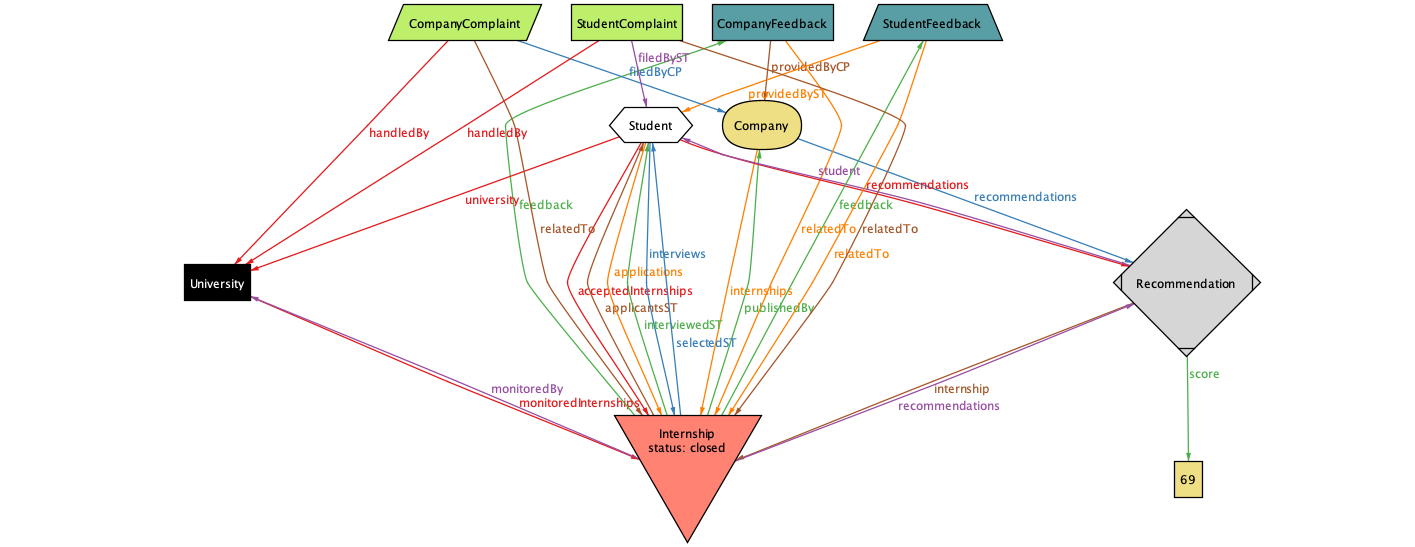
\includegraphics[width=1.2\linewidth]{Alloy/BaseWorld.png}
        \caption{Instance for \textit{BaseWorld}.}
        \label{fig:baseWorld}%
    \end{center}
\end{figure}

\begin{figure}[H]
    \begin{center}
        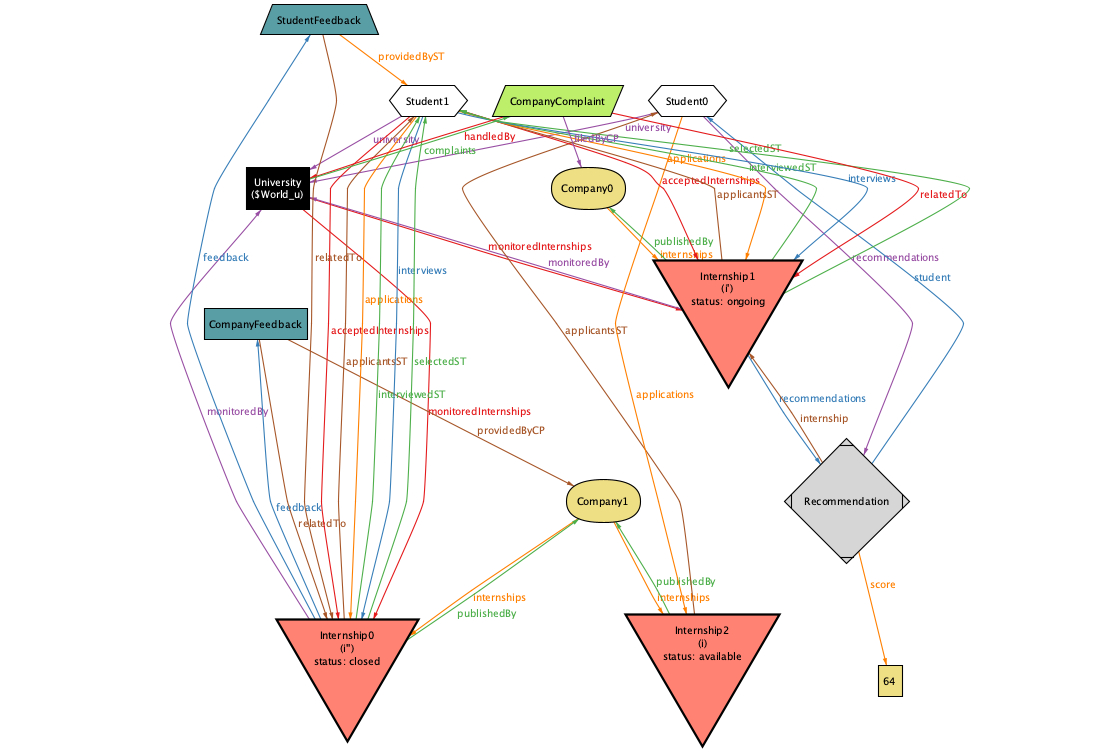
\includegraphics[width=1\linewidth]{Alloy/World1.png}
        \caption{Instance for \textit{World1}.}
        \label{fig:World1}%
    \end{center}
\end{figure}


\begin{figure}[H]
    \begin{center}
        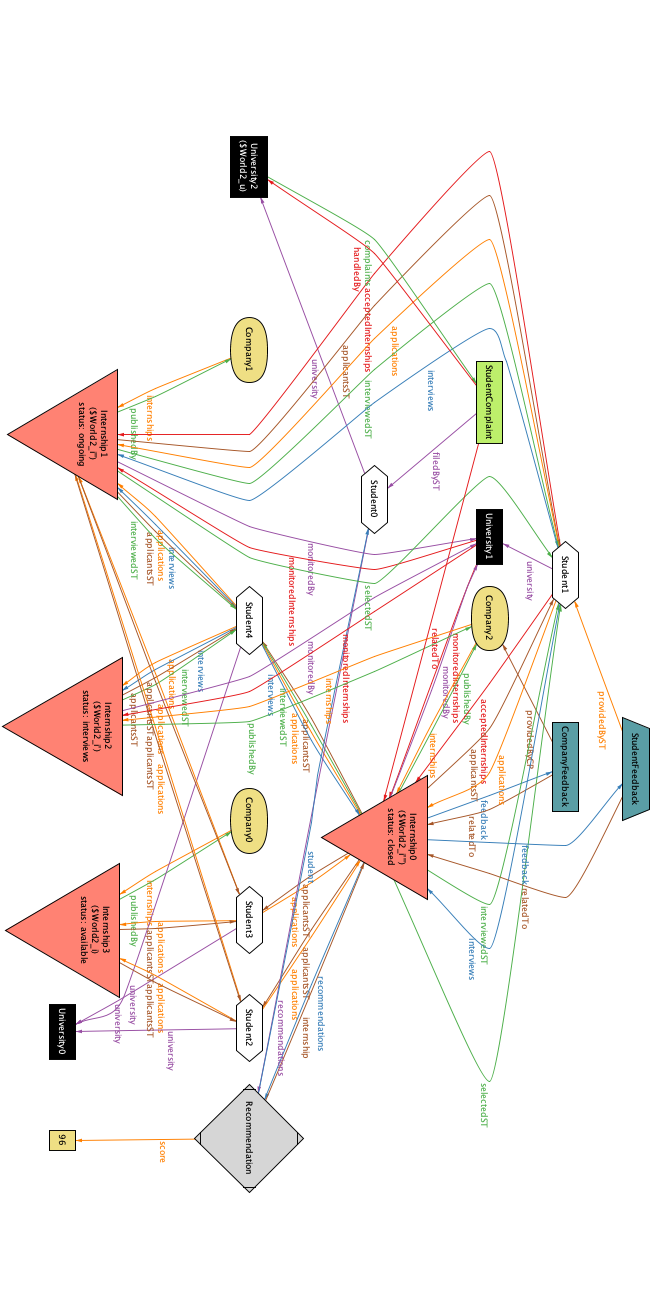
\includegraphics[width=0.8\linewidth]{Alloy/World2.png}
        \caption{Instance for \textit{World2}.}
        \label{fig:World2}%
    \end{center}
\end{figure}


    \chapter{Effort Spent}
    \label{ch:effort_spent}%
    \begin{table}[H]
    \begin{center}
        \begin{tabular}{c|c}
            \hline
            Member of group & Effort spent \\
            \hline
            Pianalto Riccardo & \begin{tabular}{p{0.25\linewidth}|c}
                             Introduction          & $1.5h$  \\
                             Overall description   & $10h$ \\
                             Specific requirements & $11h$ \\
                             Formal analysis       & $1.5h$ \\
                             Reasoning             & $3h$ \\
            \end{tabular} \\
            \hline
            Pica Mirko & \begin{tabular}{p{0.25\linewidth}|c}
                             Introduction          & $2h$  \\
                             Overall description   & $6.5h$ \\
                             Specific requirements & $9h$ \\
                             Formal analysis       & $15h$  \\
                             Reasoning             & $3.5h$ \\
            \end{tabular} \\
            \hline
            Prendin Christian & \begin{tabular}{p{0.25\linewidth}|c}
                                     Introduction          & $6h$\\
                                     Overall description   & $4h$\\
                                     Specific requirements & $2h$\\
                                     Formal analysis       & $16h$\\
                                     Reasoning             & $5h$\\
            \end{tabular} \\
            \hline
        \end{tabular}
        \caption{Effort spent by each member of the group.}
        \label{tab:effor_spent}
    \end{center}
\end{table}





    \chapter{References}
    \label{ch:references}%
    \section{References}
\label{sec:references}%

\begin{itemize}
    \item ISO/IEC/IEEE 29148:2018 - Systems and software engineering - Life cycle processes - Requirements engineering.
    \item The Requirement Engineering and Design Project specification document A.Y. 2024–2025. 
\end{itemize}

\section{Used Tools}
\label{sec:used_tools}%
\begin{itemize}
    \item \textit{GitHub} for project versioning and sharing.
    \item \LaTeX{} and \textit{Overleaf} as editor for writing this document.
    \item \textit{sequencediagram.org} for the sequence diagrams' design.
    \item \textit{Lucidchart} for the other diagrams' design.
    \item \textit{Alloy} for formal analysis.
    \item \textit{Google Docs} for collaborative writing, notes and reasoning.
\end{itemize}


% LIST OF FIGURES
    \listoffigures

% LIST OF TABLES
    \listoftables
    \cleardoublepage


\end{document}
